First in Figure \ref{fig:flow1} the fluid flow velocity is plotted. Parabolic behavious is observed closer to the edges as is expected.

Now let's see what happens to the flow if objects are placed in the flow.

In the following figures snapshots are seen depecting various objects in the horizontal pipe flow.

\begin{figure}[htb]
        \centering
        \begin{subfigure}[b]{0.4\textwidth}
                \centering
                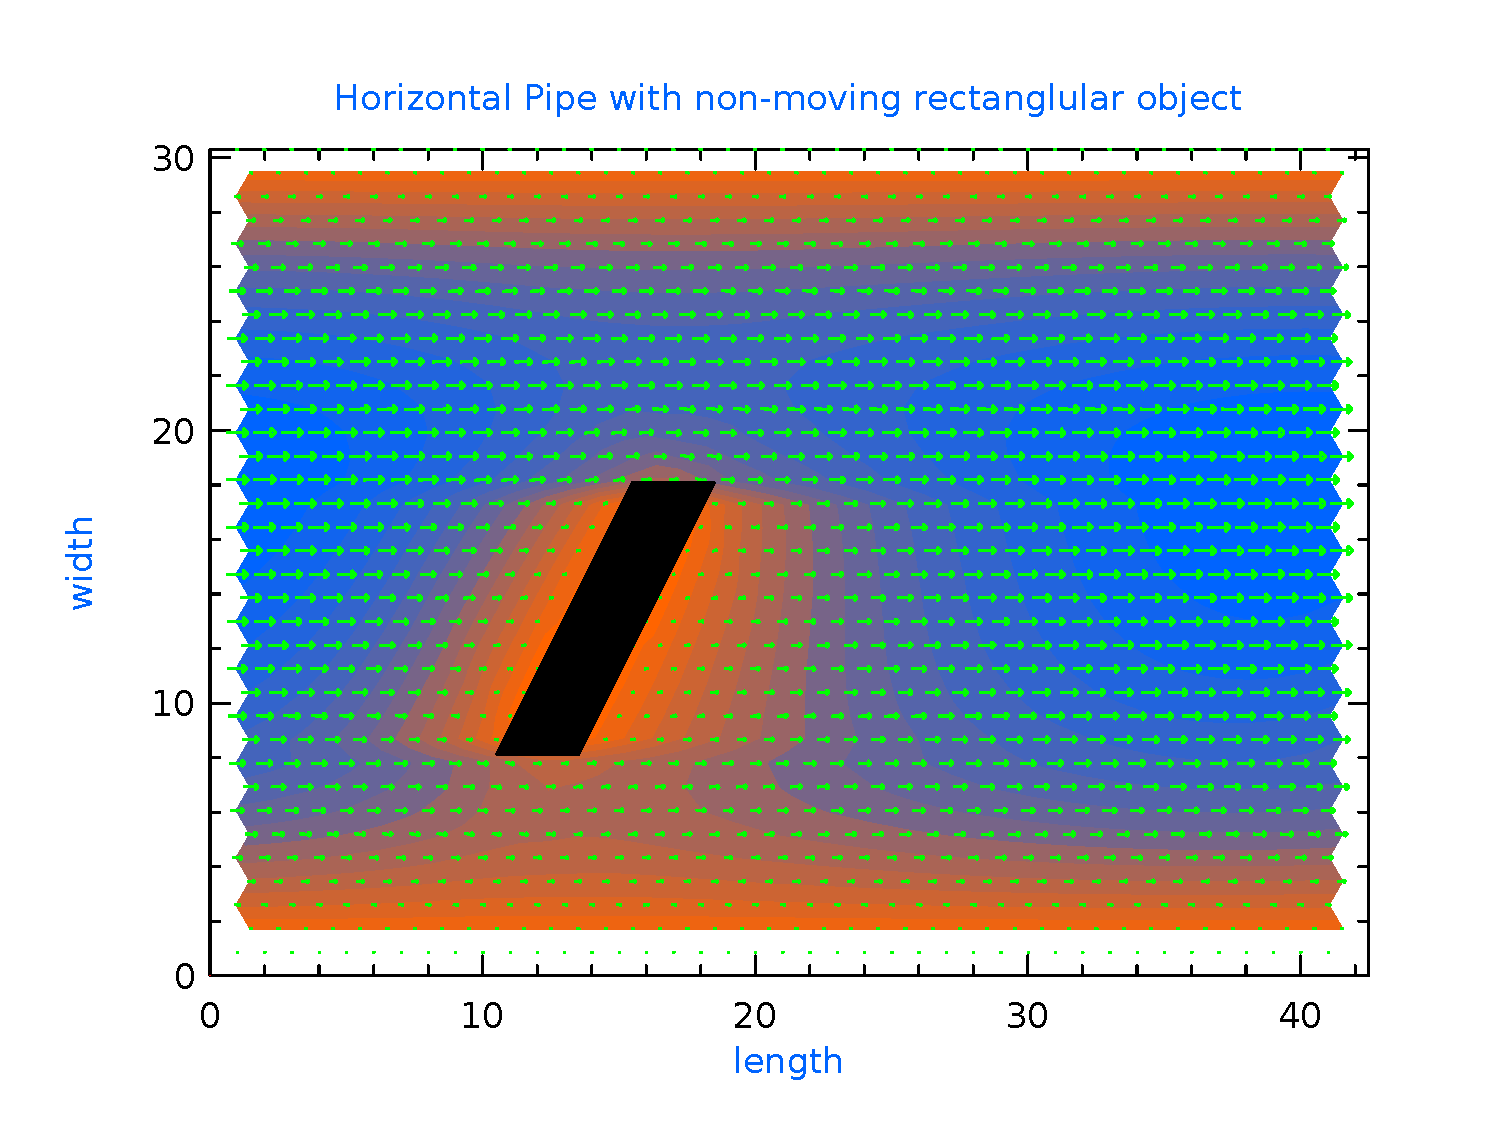
\includegraphics[width=\textwidth]{plots/rectangle.pdf}
                \caption{Non-moving rectangle placed in the laminar flow.}
                \label{fig:rectangle}
        \end{subfigure}
    \quad
        \begin{subfigure}[b]{0.4\textwidth}
                \centering
                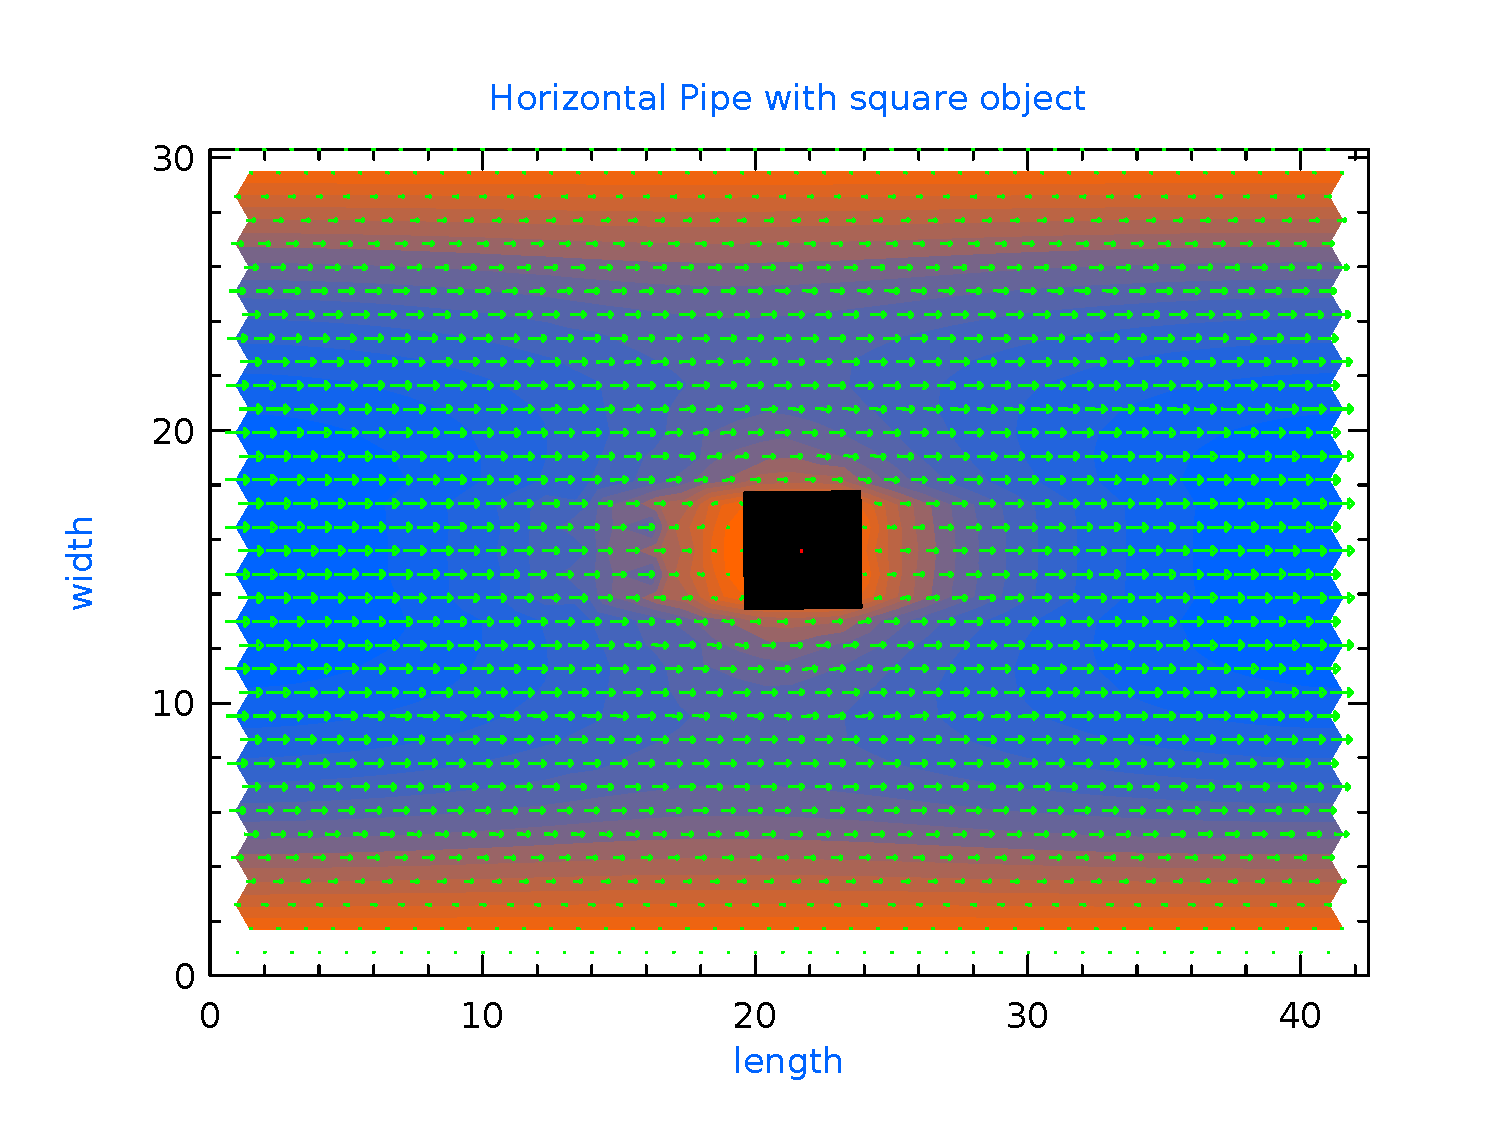
\includegraphics[width=\textwidth]{plots/square.pdf}
                \caption{Moving square placed in the laminar flow. It is placed near the middle of the flow so it hardly rotates.}
                \label{fig:rectangle}
        \end{subfigure}\\
            \begin{subfigure}[b]{0.4\textwidth}
            \centering
            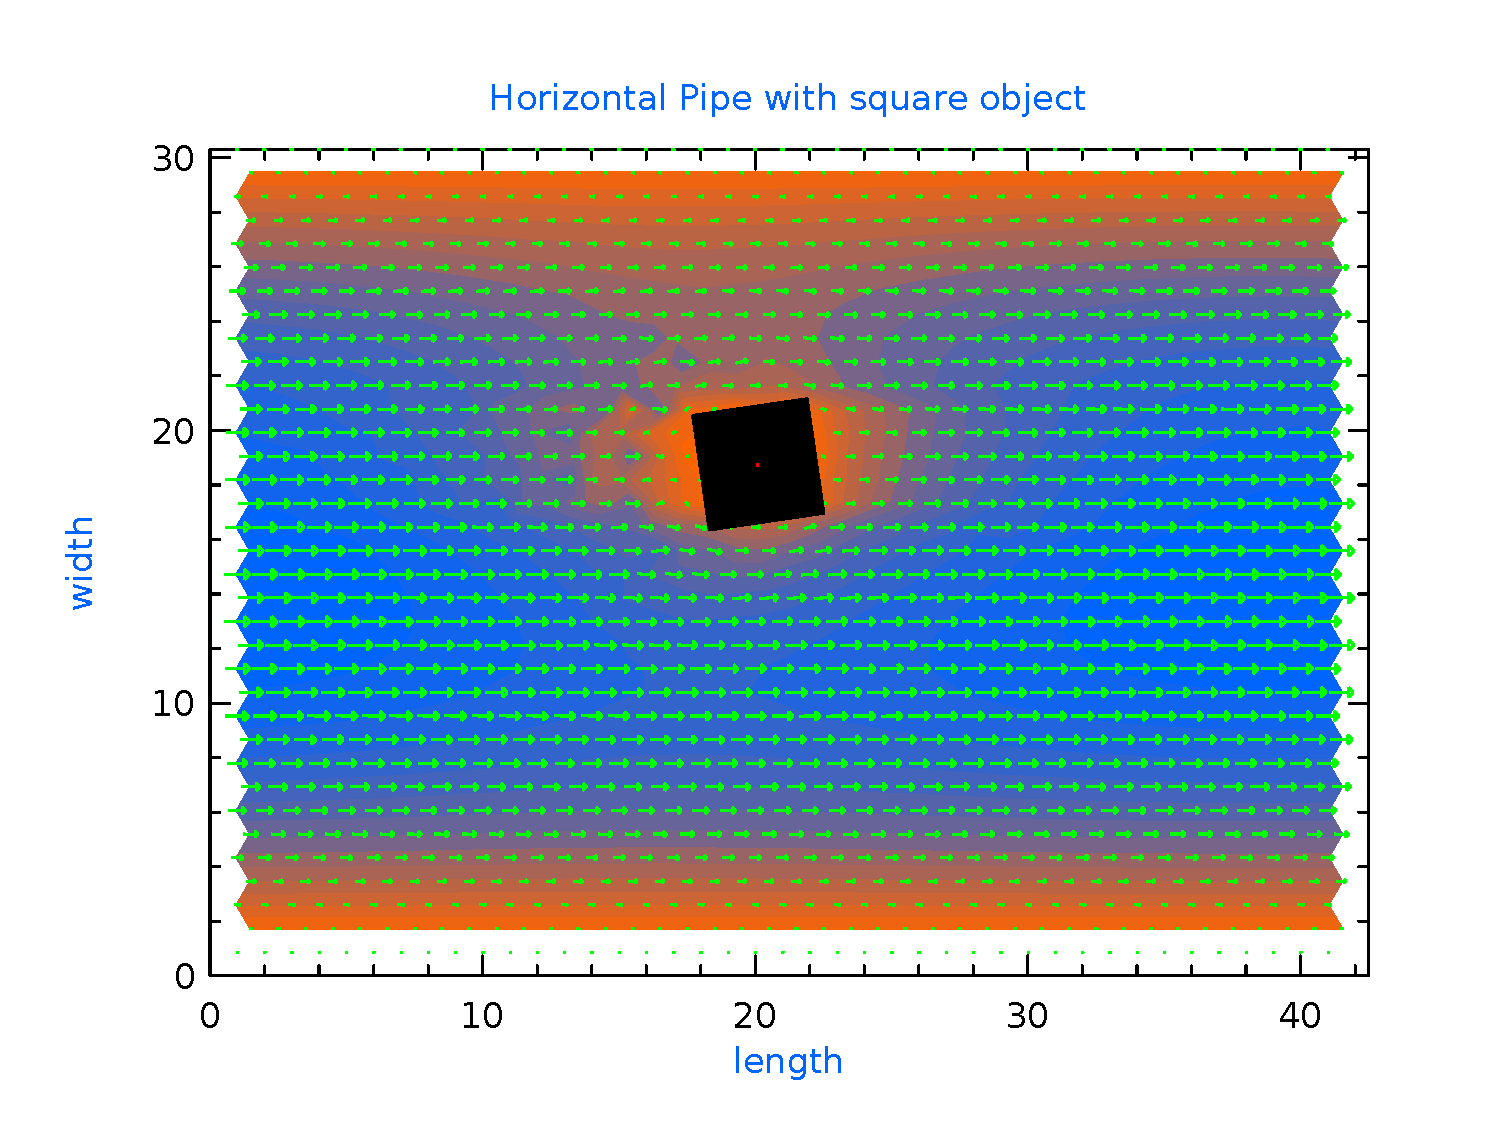
\includegraphics[width=\textwidth]{plots/rotating_square.pdf}
            \caption{Moving square placed in the laminar flow. It is placed near the edge of the flow so it rotates.}
            \label{fig:rectangle}
    \end{subfigure}
\quad
    \begin{subfigure}[b]{0.4\textwidth}
            \centering
            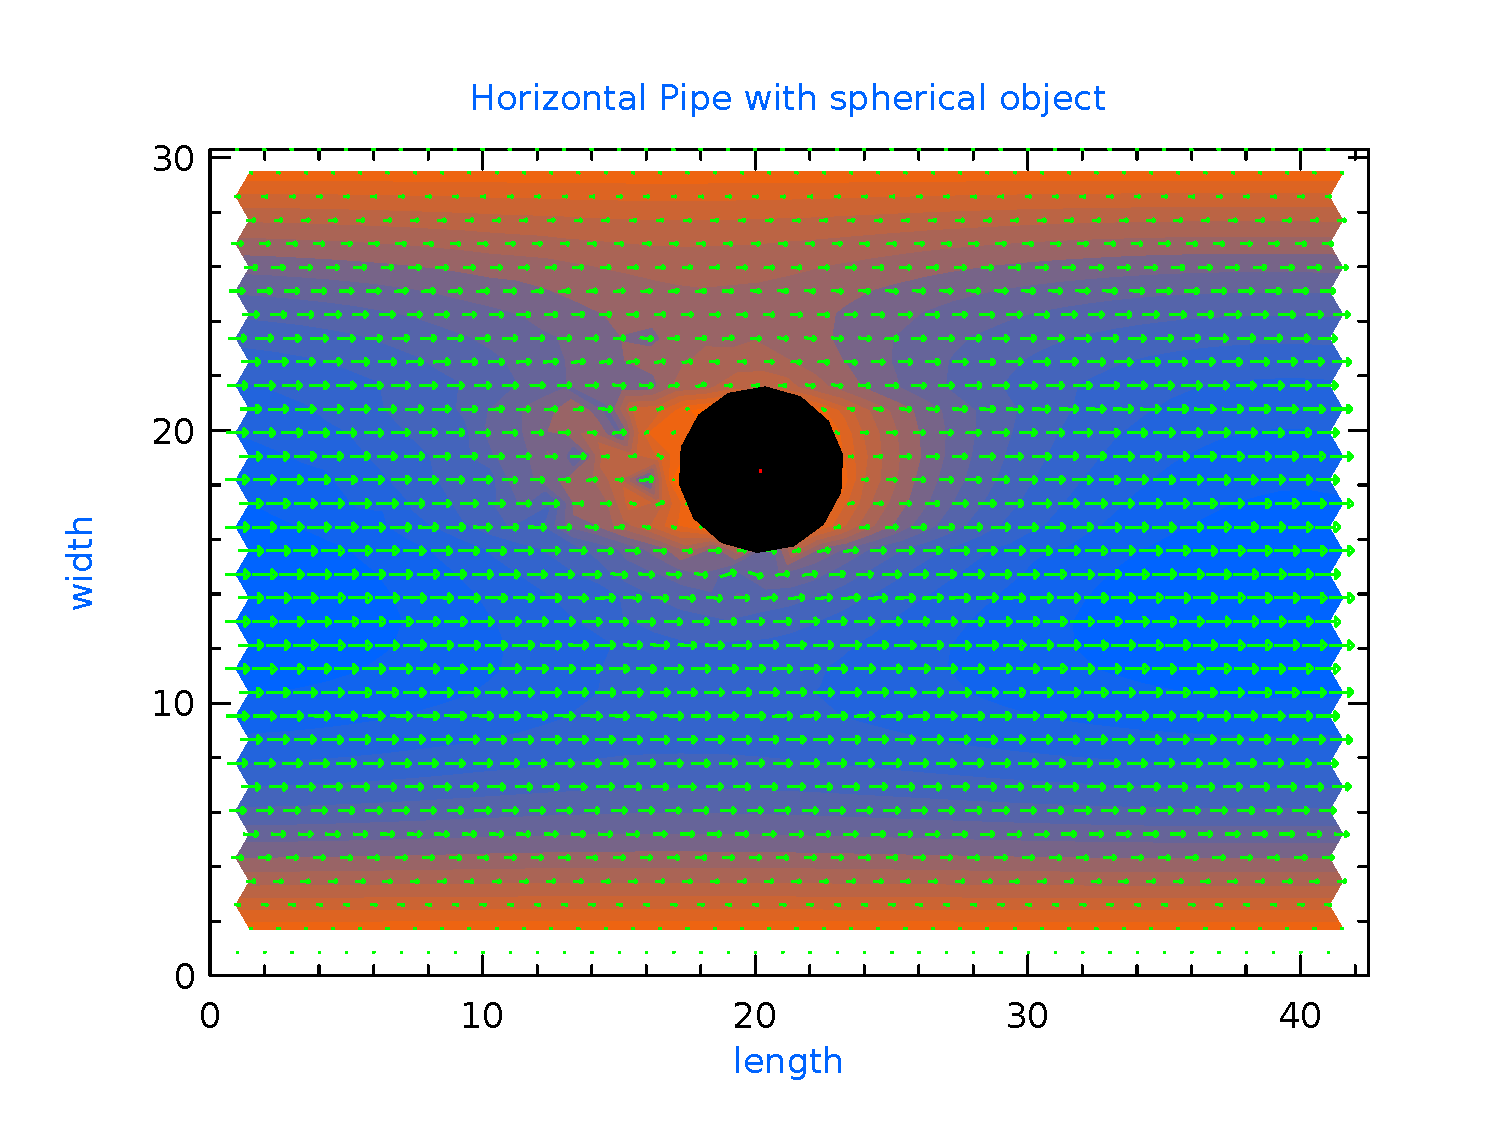
\includegraphics[width=\textwidth]{plots/sphere.pdf}
            \caption{Moving sphere placed in the laminar flow.}
            \label{fig:rectangle}
    \end{subfigure}
        \caption{Objects placed in laminar flow. The arrows give an indication of the velocity at that point, the color indicates the horizontal velocity. Low velocities correspond to orange, high velocities to blue.}
        \label{fig:flow1}
\end{figure}
